\section{锥规划}
\label{sec:cone-conic}

二次规划的约束仍是平的，可行集的边界由超平面拼成。距离上限、矩阵半正定这样的条件却给出弯曲的边界。接下来要弄清：怎样把这些弯曲的约束放进一个共同的形式，同时保留线性规划那种“任何人都能核对”的对偶下界？

\paragraph{从非负约束到锥约束}
回看第~\ref{chap:linear-programming}章的线性规划
\[
 \min_{\bm{x}}\ \bm{c}^\top\bm{x}\quad\text{s.t.}\quad\bm{A}\bm{x}=\bm{b},\quad\bm{x}\geq\bm{0}.
\]
目标和等式都是线性的，问题的全部“形状”集中在一条约束上：$\bm{x}$属于非负象限$\mathbb{R}^n_+$。

对偶理论用到非负象限的什么性质？只有三条：它是闭集，它是凸集，它对乘以非负数封闭。保留这三条，把非负象限换成别的集合，线性规划的框架就可以搬过去。

\begin{definition}[闭凸锥]
\label{def:cone-closed-convex-cone}
设$\bm{K}\subseteq\mathbb{R}^N$非空。若$\bm{K}$是闭凸集，且对任意$\bm{x}\in\bm{K}$和$\theta\geq0$都有$\theta\bm{x}\in\bm{K}$，则称$\bm{K}$是\term{闭凸锥}（closed convex cone）。
\end{definition}

非负象限是闭凸锥。闭单位球不是，因为把球内的点放大后会跑到球外。两条相交直线的并也不是，它对放缩封闭，但不凸。

现在让仿射表达式属于这样的锥，就得到下面的共同形式。

\begin{definition}[锥规划]
\label{def:cone-conic-program}
设$\bm{K}\subseteq\mathbb{R}^N$是闭凸锥，$\bm{c}\in\mathbb{R}^n$，$\bm{A}\in\mathbb{R}^{p\times n}$，$\bm{b}\in\mathbb{R}^p$，$\bm{E}\in\mathbb{R}^{N\times n}$，$\bm{g}\in\mathbb{R}^N$。问题
\begin{equation}
 \min_{\bm{x}}\ \bm{c}^\top\bm{x}\quad\text{s.t.}\quad\bm{A}\bm{x}=\bm{b},\quad\bm{E}\bm{x}+\bm{g}\in\bm{K}
 \label{eq:cone-conic}
\end{equation}
称为\term{锥规划}（conic program）。$\bm{K}$可以是若干个锥的直积，此时每一块分别属于对应的锥。
\end{definition}

取$\bm{K}=\mathbb{R}^n_+$、$\bm{E}=\bm{I}$、$\bm{g}=\bm{0}$，得到线性规划。目标依然是线性的，等式依然是线性的，全部非线性都收进了“属于$\bm{K}$”这一句话。

可以把“$\bm{E}\bm{x}+\bm{g}\in\bm{K}$”读成广义的“大于等于零”。这个类比在一处失效：实数总能比较大小，一般的锥却给不出全序，$\bm{v}$和$-\bm{v}$可能都不属于$\bm{K}$。于是下面的乘子也不能再简单地说成“非负”。

\paragraph{对偶锥}
线性规划的对偶之所以成立，是因为$\bm{x}\geq\bm{0}$、$\bm{s}\geq\bm{0}$时必有$\bm{s}^\top\bm{x}\geq0$。换成一般的锥，要问：什么样的向量$\bm{s}$与$\bm{K}$中每个向量的内积都非负？

\begin{definition}[对偶锥]
\label{def:cone-dual-cone}
闭凸锥$\bm{K}\subseteq\mathbb{R}^N$的\term{对偶锥}（dual cone）是
\begin{equation}
 \bm{K}^*=\{\bm{s}\in\mathbb{R}^N:\langle\bm{s},\bm{x}\rangle\geq0\text{ 对所有 }\bm{x}\in\bm{K}\text{ 成立}\}.
 \label{eq:cone-dual-cone}
\end{equation}
\end{definition}

把$\bm{s}$看成一组价格，$\bm{x}\in\bm{K}$看成一份允许的持仓，$\langle\bm{s},\bm{x}\rangle$就是持仓的价值。对偶锥里的价格保证：无论持有$\bm{K}$中哪一份，价值都不为负。这个类比的边界在于，价格的单个分量可以是负的，只要$\bm{K}$中的向量不会让总价值变负就行。

图~\ref{fig:cone-dual-cones}画出平面上的三个例子，几何上$\bm{K}^*$由与$\bm{K}$中所有方向夹角不超过直角的方向组成。

\begin{BookInlineFigure}
  \centering
  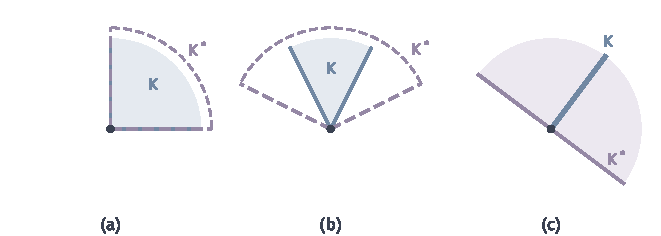
\includegraphics[width=112mm]{figures/05-optimization/06-constrained-optimization/matplotlib/cone-dual-cones/figure.pdf}
  \caption{平面上的锥（蓝色）与对偶锥（紫色）。(a)第一象限的对偶锥是它自身，紫色虚线与蓝色边界重合。(b)窄锥$\{(u,t):\lvert u\rvert\leq t/2\}$的对偶锥是宽锥$\{(v,w):\lvert v\rvert\leq2w\}$。(c)一条射线的对偶锥是一个闭半平面。各锥只画出原点附近的一部分。}
  \label{fig:cone-dual-cones}
\end{BookInlineFigure}

(b)可以手算。设$\bm{K}=\{(u,t):\lvert u\rvert\leq t/2\}$，对$(v,w)$要求$vu+wt\geq0$对所有$\bm{K}$中的点成立。固定$t\geq0$，左端在$u=\pm t/2$中使$vu$为负的那一端最小，最小值是
\[
 -\lvert v\rvert\frac{t}{2}+wt=t\Bigl(w-\frac{\lvert v\rvert}{2}\Bigr).
\]
它对所有$t\geq0$非负，当且仅当$\lvert v\rvert\leq2w$。$\bm{K}$越窄，需要照顾的方向越少，$\bm{K}^*$就越宽。

\paragraph{下界与证书}
第~\ref{chap:duality}章的做法是：把约束乘上乘子加进目标，再对$\bm{x}$取下确界，得到最优值的下界。这里用同样的计算，只是把“非负乘子”换成“对偶锥中的乘子”。

取$\bm{y}\in\mathbb{R}^p$和$\bm{s}\in\bm{K}^*$，构造
\[
 \mathcal{L}(\bm{x},\bm{y},\bm{s})=\bm{c}^\top\bm{x}+\bm{y}^\top(\bm{b}-\bm{A}\bm{x})-\bm{s}^\top(\bm{E}\bm{x}+\bm{g}).
\]
可行的$\bm{x}$满足$\bm{b}-\bm{A}\bm{x}=\bm{0}$，且$\bm{s}^\top(\bm{E}\bm{x}+\bm{g})\geq0$，所以$\mathcal{L}\leq\bm{c}^\top\bm{x}$。

$\mathcal{L}$对$\bm{x}$是仿射的，$\bm{x}$的系数必须为零，下确界才不是$-\infty$。这个条件是$\bm{A}^\top\bm{y}+\bm{E}^\top\bm{s}=\bm{c}$，此时下确界等于$\bm{b}^\top\bm{y}-\bm{g}^\top\bm{s}$。于是得到\term{锥对偶问题}（conic dual problem）
\begin{equation}
 \max_{\bm{y},\bm{s}}\ \bm{b}^\top\bm{y}-\bm{g}^\top\bm{s}\quad\text{s.t.}\quad\bm{A}^\top\bm{y}+\bm{E}^\top\bm{s}=\bm{c},\quad\bm{s}\in\bm{K}^*.
 \label{eq:cone-conic-dual}
\end{equation}

\begin{theorem}[锥规划的弱对偶]
\label{thm:cone-weak-duality}
设$\bm{x}$是问题~\eqref{eq:cone-conic}的可行点，$(\bm{y},\bm{s})$是问题~\eqref{eq:cone-conic-dual}的可行点，则
\begin{equation}
 \bm{c}^\top\bm{x}-(\bm{b}^\top\bm{y}-\bm{g}^\top\bm{s})=\bm{s}^\top(\bm{E}\bm{x}+\bm{g})\geq0.
 \label{eq:cone-conic-gap}
\end{equation}
\end{theorem}

\begin{proof}
把$\bm{c}=\bm{A}^\top\bm{y}+\bm{E}^\top\bm{s}$代入$\bm{c}^\top\bm{x}$，并用$\bm{A}\bm{x}=\bm{b}$，得到
\[
 \bm{c}^\top\bm{x}=\bm{y}^\top\bm{b}+\bm{s}^\top\bm{E}\bm{x}.
\]
两边减去$\bm{b}^\top\bm{y}-\bm{g}^\top\bm{s}$，右端成为$\bm{s}^\top(\bm{E}\bm{x}+\bm{g})$。由$\bm{s}\in\bm{K}^*$和$\bm{E}\bm{x}+\bm{g}\in\bm{K}$，它非负。
\end{proof}

式~\eqref{eq:cone-conic-gap}的用法是：手里有一个原始可行点和一个对偶可行点，最优值就被夹在两个目标值之间。若两个值相等，两个点同时最优。这个判断只用到可行性和内积，不需要知道它们是怎么算出来的。

对线性规划，$\bm{K}^*=\mathbb{R}^n_+$，问题~\eqref{eq:cone-conic-dual}就是第~\ref{chap:linear-programming}章的对偶问题，式~\eqref{eq:cone-conic-gap}就是$\bm{s}^\top\bm{x}\geq0$。

\subsection{二阶锥规划}
\label{sec:cone-socp}

“到某点的距离不超过某个值”是最常见的弯曲约束。这一小节要把它写进锥规划，并弄清右端的符号在其中起什么作用。

\paragraph{二阶锥}
距离上限的形状是一个圆盘。把半径$t$也当作变量，圆盘就随高度放大，叠起来成为一个圆锥。

\begin{definition}[二阶锥规划]
\label{def:cone-socp}
集合
\begin{equation}
 \bm{K}_{\mathrm{so}}^{k+1}=\{(\bm{u},t)\in\mathbb{R}^k\times\mathbb{R}:\lVert\bm{u}\rVert_2\leq t\}
 \label{eq:cone-soc}
\end{equation}
称为\term{二阶锥}（second-order cone）。问题
\begin{equation}
 \begin{aligned}
 \min_{\bm{x}}\quad&\bm{q}^\top\bm{x}\\
 \text{s.t.}\quad&\lVert\bm{A}_i\bm{x}+\bm{b}_i\rVert_2\leq\bm{c}_i^\top\bm{x}+d_i,\quad i=1,\ldots,m,\\
 &\bm{A}\bm{x}=\bm{b}
 \end{aligned}
 \label{eq:cone-socp}
\end{equation}
称为\term{二阶锥规划}（second-order cone program，SOCP）。这里$\bm{A}_i\in\mathbb{R}^{k_i\times n}$，$\bm{b}_i\in\mathbb{R}^{k_i}$，$\bm{c}_i\in\mathbb{R}^n$，$d_i\in\mathbb{R}$。
\end{definition}

第$i$条约束说的正是
\[
 (\bm{A}_i\bm{x}+\bm{b}_i,\ \bm{c}_i^\top\bm{x}+d_i)\in\bm{K}_{\mathrm{so}}^{k_i+1}.
\]

这个集合确实是闭凸锥。放缩时范数按倍数变化，$\theta\geq0$时仍有$\lVert\theta\bm{u}\rVert_2\leq\theta t$；相加时由三角不等式，
\[
 \lVert\bm{u}_1+\bm{u}_2\rVert_2\leq\lVert\bm{u}_1\rVert_2+\lVert\bm{u}_2\rVert_2\leq t_1+t_2.
\]
放缩和相加封闭，合起来就是凸。闭性来自范数连续。

图~\ref{fig:cone-soc-3d}画出$k=2$时的二阶锥，高度为$t$的水平截面是半径为$t$的圆盘。

\begin{BookInlineFigure}
  \centering
  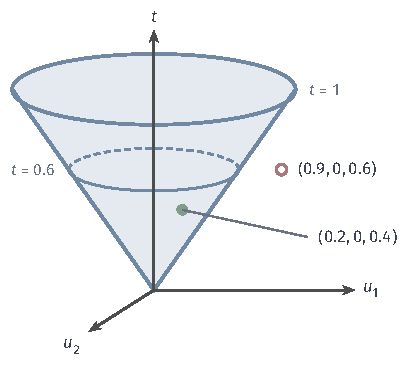
\includegraphics[width=66mm]{figures/05-optimization/06-constrained-optimization/tikz/cone-soc-3d/figure.pdf}
  \caption{$\mathbb{R}^3$中的二阶锥$\sqrt{u_1^2+u_2^2}\leq t$，画出$0\leq t\leq1$的部分。绿点$(0.2,0,0.4)$满足$0.2\leq0.4$，在锥内。红色空心点$(0.9,0,0.6)$不满足$0.9\leq0.6$，在锥外。}
  \label{fig:cone-soc-3d}
\end{BookInlineFigure}

\paragraph{右端非负也是条件的一部分}
约束的左端是范数，总是非负的，所以满足约束就迫使$\bm{c}_i^\top\bm{x}+d_i\geq0$。这个隐含的符号条件不可丢弃。

有人会想两边平方，把约束写成$\lVert\bm{u}\rVert_2^2\leq t^2$。这一步改变了集合。正确的等价关系是
\begin{equation}
 \lVert\bm{u}\rVert_2\leq t\quad\Longleftrightarrow\quad t\geq0\text{ 且 }\lVert\bm{u}\rVert_2^2\leq t^2.
 \label{eq:cone-soc-square}
\end{equation}
去掉$t\geq0$后，$(u,t)=(1,-2)$满足$1\leq4$，却不满足$1\leq-2$。

图~\ref{fig:cone-soc-square}对比了两个集合。平方之后得到的是上下两片，这个集合甚至不凸。

\begin{BookInlineFigure}
  \centering
  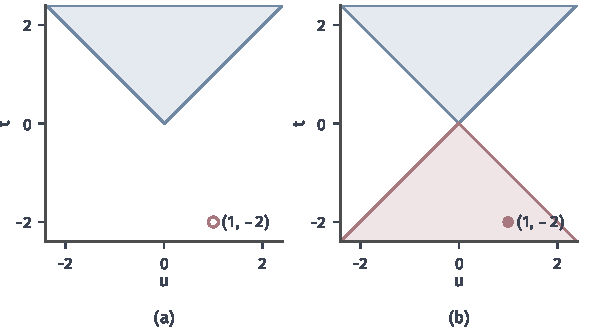
\includegraphics[width=100mm]{figures/05-optimization/06-constrained-optimization/matplotlib/cone-soc-square/figure.pdf}
  \caption{平方丢失符号信息。(a)二阶锥$\lvert u\rvert\leq t$，点$(1,-2)$不在其中。(b)$u^2\leq t^2$的解集多出了红色的下半部分，点$(1,-2)$落在其中，集合不再是凸集。}
  \label{fig:cone-soc-square}
\end{BookInlineFigure}

\paragraph{距离上限的交集}
下面用一个能手算的例子看这类可行集。在两个圆盘的公共部分里求最低的点：
\begin{equation}
 \min_{\bm{x}\in\mathbb{R}^2}\ x_2\quad\text{s.t.}\quad\lVert\bm{x}-\bm{a}_1\rVert_2\leq5,\quad\lVert\bm{x}-\bm{a}_2\rVert_2\leq5,
 \label{eq:cone-lens}
\end{equation}
其中$\bm{a}_1=(0,0)$，$\bm{a}_2=(6,0)$。对照式~\eqref{eq:cone-socp}，$\bm{q}=(0,1)$，$\bm{A}_i=\bm{I}$，$\bm{b}_i=-\bm{a}_i$，$\bm{c}_i=\bm{0}$，$d_i=5$。

每条约束是一个圆盘，二者的交仍是凸集，形状像一枚透镜，如图~\ref{fig:cone-soc-lens}所示。它的边界是弯的，所以不是多面体，线性规划和二次规划的可行集都表达不了。

\begin{BookInlineFigure}
  \centering
  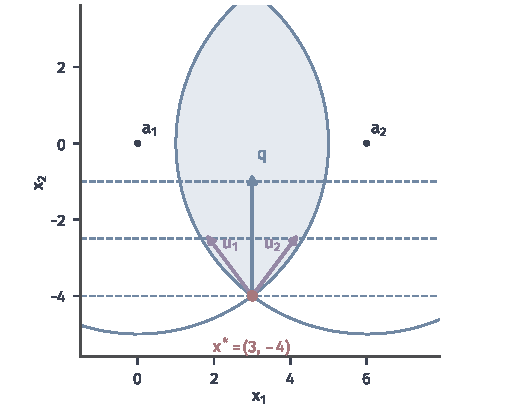
\includegraphics[width=88mm]{figures/05-optimization/06-constrained-optimization/matplotlib/cone-soc-lens/figure.pdf}
  \caption{两条距离约束的交集。浅蓝透镜是可行集，蓝色虚线是目标$x_2$的等值线，红点是解$(3,-4)$。紫色箭头是第~\ref{sec:cone-duality-certificates}小节算出的乘子分量$\bm{u}_1,\bm{u}_2$，蓝色箭头是目标系数$\bm{q}=\bm{u}_1+\bm{u}_2$，三者同乘$3.2$后画出。}
  \label{fig:cone-soc-lens}
\end{BookInlineFigure}

透镜的最低点是两个圆的交点。把两个圆的方程相减，
\[
 x_1^2+x_2^2-(x_1-6)^2-x_2^2=0,
\]
化简得$x_1=3$。代回第一个圆，得到$x_2=\pm4$。所以候选解是$(3,-4)$，目标值$-4$。它确实最优，稍后用对偶解来证明。

\paragraph{右端含变量}
约束右端也可以依赖决策变量。设要找一个位置$\bm{x}$，使它到三个站点的最大距离最小。引入变量$t$表示这个最大距离，问题写成
\begin{equation}
 \min_{\bm{x},t}\ t\quad\text{s.t.}\quad\lVert\bm{x}-\bm{p}_i\rVert_2\leq t,\quad i=1,2,3.
 \label{eq:cone-enclosing}
\end{equation}
这里决策变量是$(\bm{x},t)\in\mathbb{R}^3$，每条约束的右端$\bm{c}_i^\top(\bm{x},t)+d_i$就是$t$。在$(\bm{x},t)$空间里，每条约束是一个顶点在$(\bm{p}_i,0)$的圆锥，可行集是三个圆锥的交。

取$\bm{p}_1=(0,0)$，$\bm{p}_2=(6,0)$，$\bm{p}_3=(3,9)$。点$\bm{x}^\star=(3,4)$到三个站点的距离都是$5$，图~\ref{fig:cone-soc-enclosing}(a)是相应的覆盖圆。

\begin{BookInlineFigure}
  \centering
  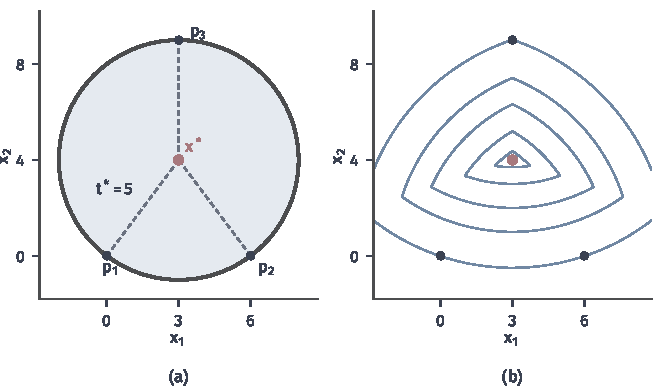
\includegraphics[width=112mm]{figures/05-optimization/06-constrained-optimization/matplotlib/cone-soc-enclosing/figure.pdf}
  \caption{最小化到三个站点的最大距离。(a)红点到三个站点的距离都等于$t^\star=5$，深灰圆是覆盖三点的最小圆。(b)蓝线是函数$\max_i\lVert\bm{x}-\bm{p}_i\rVert_2$的等高线，三段圆弧在折角处相接，目标不可微，而写成式~\eqref{eq:cone-enclosing}后目标和约束都很规则。}
  \label{fig:cone-soc-enclosing}
\end{BookInlineFigure}

下面验证$\bm{x}^\star$最优。三个站点相对$\bm{x}^\star$的位置是$(-3,-4)$、$(3,-4)$、$(0,5)$，用正权重$5,5,8$加权，和为零：
\[
 5\begin{bmatrix}-3\\-4\end{bmatrix}+5\begin{bmatrix}3\\-4\end{bmatrix}+8\begin{bmatrix}0\\5\end{bmatrix}=\bm{0}.
\]
所以对任何位移$\bm{d}\neq\bm{0}$，三个数$\bm{d}^\top(\bm{p}_i-\bm{x}^\star)$不可能全部非负且不全为零；又因三个向量张成平面，它们也不会全为零。因此总有某个$i$使$\bm{d}^\top(\bm{p}_i-\bm{x}^\star)<0$。

对这个$i$，位移后的距离满足
\[
 \lVert\bm{x}^\star+\bm{d}-\bm{p}_i\rVert_2^2=25+\lVert\bm{d}\rVert_2^2-2\bm{d}^\top(\bm{p}_i-\bm{x}^\star)>25.
\]
最大距离严格变大，所以$\bm{x}^\star$是唯一的最优位置，$t^\star=5$。

\subsection{半正定规划}
\label{sec:cone-sdp}

有些量天然是矩阵，而且必须像协方差矩阵那样半正定。这一小节回答：矩阵半正定的约束怎样放进锥规划，它能表达哪些条件，又怎样用特征值检验？

\paragraph{矩阵作变量}
记$\mathcal{S}^n$为$n\times n$实对称矩阵组成的线性空间。在其上使用\term{迹内积}（trace inner product）
\begin{equation}
 \langle\bm{X},\bm{Y}\rangle=\operatorname{tr}(\bm{X}\bm{Y})=\sum_{i,j}X_{i,j}Y_{i,j}.
 \label{eq:cone-trace-inner}
\end{equation}
把矩阵按元素排成长向量，这就是普通的欧氏内积。

半正定矩阵的集合记为$\mathcal{S}^n_+$。$\bm{X}\in\mathcal{S}^n_+$的定义是对所有$\bm{v}$有$\bm{v}^\top\bm{X}\bm{v}\geq0$，等价于全部特征值非负，这个等价关系可参考\BookChapterRef{chap:eigen-spectral-decomposition}{卷二第6章“谱分解”}。

$\mathcal{S}^n_+$是闭凸锥。对固定的$\bm{v}$，$\bm{v}^\top\bm{X}\bm{v}\geq0$是$\bm{X}$的一个线性不等式，定义的是过原点的闭半空间。$\mathcal{S}^n_+$是无穷多个这样的闭半空间的交，所以它闭、凸，且对非负放缩封闭。

\begin{definition}[半正定规划]
\label{def:cone-sdp}
给定$\bm{W},\bm{A}_1,\ldots,\bm{A}_m\in\mathcal{S}^n$和$\bm{b}\in\mathbb{R}^m$，问题
\begin{equation}
 \begin{aligned}
 \min_{\bm{X}\in\mathcal{S}^n}\quad&\langle\bm{W},\bm{X}\rangle\\
 \text{s.t.}\quad&\langle\bm{A}_i,\bm{X}\rangle=b_i,\quad i=1,\ldots,m,\\
 &\bm{X}\succeq\bm{0}
 \end{aligned}
 \label{eq:cone-sdp}
\end{equation}
称为\term{半正定规划}（semidefinite program，SDP）。$\bm{X}\succeq\bm{0}$表示$\bm{X}\in\mathcal{S}^n_+$。
\end{definition}

\paragraph{半正定不是逐元素非负}
“$\bm{X}\succeq\bm{0}$”和“$\bm{X}$的元素非负”容易混淆，其实二者互不包含。$\begin{bmatrix}1&2\\2&1\end{bmatrix}$元素全正，特征值却有$-1$。$\begin{bmatrix}1&-1\\-1&1\end{bmatrix}$有负元素，特征值是$0$和$2$，半正定。

为了看清这个差别，取迹为$1$的$2\times2$对称矩阵
\[
 \bm{X}=\begin{bmatrix}a&b\\b&1-a\end{bmatrix}.
\]
$2\times2$矩阵半正定，当且仅当两个对角元和行列式都非负。这里就是$a(1-a)-b^2\geq0$，配方得到
\[
 \Bigl(a-\frac12\Bigr)^2+b^2\leq\frac14.
\]
半正定的矩阵组成一个圆盘，而逐元素非负的要求是一条竖带的上半部分，见图~\ref{fig:cone-sdp-disk}。

\begin{BookInlineFigure}
  \centering
  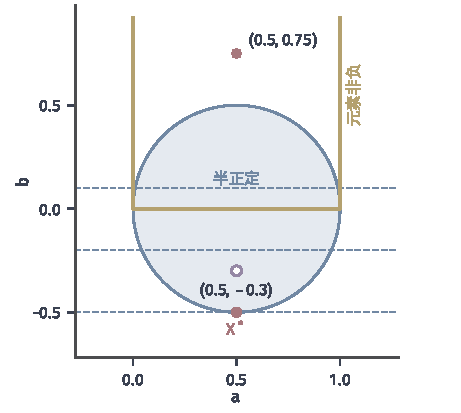
\includegraphics[width=78mm]{figures/05-optimization/06-constrained-optimization/matplotlib/cone-sdp-disk/figure.pdf}
  \caption{迹为$1$的$2\times2$对称矩阵$\begin{bmatrix}a&b\\b&1-a\end{bmatrix}$。浅蓝圆盘是半正定矩阵，黄线围住的是逐元素非负的矩阵。红色方块$(0.5,0.75)$元素非负但不半正定，紫色空心点$(0.5,-0.3)$半正定但有负元素。蓝色虚线是目标$2+2b$的等值线，红点是最优矩阵$\bm{X}^\star$。}
  \label{fig:cone-sdp-disk}
\end{BookInlineFigure}

可行集的边界是圆，所以半正定规划的最优解一般不在有限个候选的“顶点”上。在这个切片上取$\bm{W}=\begin{bmatrix}2&1\\1&2\end{bmatrix}$，最小化$\langle\bm{W},\bm{X}\rangle$，约束是$\operatorname{tr}\bm{X}=1$、$\bm{X}\succeq\bm{0}$。按式~\eqref{eq:cone-trace-inner}计算，
\[
 \langle\bm{W},\bm{X}\rangle=2a+2b+2(1-a)=2+2b.
\]
目标只依赖$b$，最小值在圆盘最低点$(a,b)=(1/2,-1/2)$取得，最优值是$1$，这正是$\bm{W}$的最小特征值。最优矩阵是
\[
 \bm{X}^\star=\frac12\begin{bmatrix}1&-1\\-1&1\end{bmatrix}.
\]

\paragraph{线性矩阵不等式}
实际问题常把变量放在矩阵的元素上，得到下面的约束：
\begin{equation}
 \bm{F}_0+x_1\bm{F}_1+\cdots+x_n\bm{F}_n\succeq\bm{0},
 \label{eq:cone-lmi}
\end{equation}
其中$\bm{F}_j\in\mathcal{S}^k$。这称为\term{线性矩阵不等式}（linear matrix inequality，LMI）。它正是式~\eqref{eq:cone-conic}中取$\bm{K}=\mathcal{S}^k_+$的情形，$\bm{E}\bm{x}+\bm{g}$是$\bm{x}$的仿射函数，取值为矩阵。

一条线性矩阵不等式可以表达弯曲的集合。例如
\[
 \bm{F}(\bm{x})=\begin{bmatrix}1+x_1&x_2\\x_2&1-x_1\end{bmatrix}
\]
的特征值是$1\pm\lVert\bm{x}\rVert_2$，所以$\bm{F}(\bm{x})\succeq\bm{0}$恰好是单位圆盘。

检验一个点是否可行，只需算特征值。取$\bm{x}=(0.6,0.6)$，特征值约为$0.152$和$1.849$，都为正，可行。取$\bm{x}=(0.8,0.8)$，最小特征值约为$-0.131$，不可行。图~\ref{fig:cone-sdp-lmi}(a)画出这两个点。

\begin{BookInlineFigure}
  \centering
  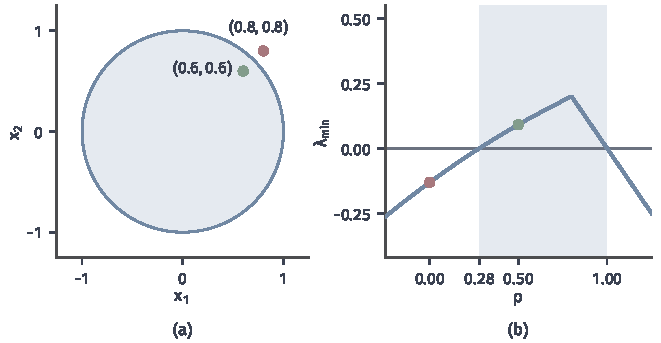
\includegraphics[width=112mm]{figures/05-optimization/06-constrained-optimization/matplotlib/cone-sdp-lmi/figure.pdf}
  \caption{用特征值检验线性矩阵不等式。(a)$\bm{F}(\bm{x})\succeq\bm{0}$的解集是单位圆盘，绿点可行，红点不可行。(b)相关矩阵~\eqref{eq:cone-corr-matrix}的最小特征值随$\rho$的变化，浅蓝区间$[0.28,1]$是使矩阵半正定的$\rho$。绿点$\rho=0.5$可行，红点$\rho=0$不可行。}
  \label{fig:cone-sdp-lmi}
\end{BookInlineFigure}

\paragraph{协方差约束}
线性矩阵不等式的一个典型来源是协方差矩阵必须半正定。设三个量两两的相关系数中，已知$\rho_{1,2}=\rho_{2,3}=0.8$，问$\rho_{1,3}=\rho$能取哪些值。相关矩阵是
\begin{equation}
 \bm{R}(\rho)=\begin{bmatrix}1&0.8&\rho\\0.8&1&0.8\\\rho&0.8&1\end{bmatrix}.
 \label{eq:cone-corr-matrix}
\end{equation}
协方差矩阵半正定这一事实的来源可参考\BookChapterRef{chap:random-vectors}{卷七第2章“随机向量与联合分布”}。这里只用到结论：$\bm{R}(\rho)$不半正定，就不存在这样的三个随机变量。

取$\rho=0$，矩阵的元素都非负，特征值却约为$-0.131$、$1$和$2.131$。所以$\rho=0$不可能，1与2强相关、2与3强相关时，1与3不能不相关。

取$\rho=0.5$，特征值约为$0.091$、$0.5$和$2.409$，可行。一般地，
\[
 \det\bm{R}(\rho)=-(\rho-1)(\rho-0.28),
\]
结合$\lvert\rho\rvert\leq1$可知可行范围是$0.28\leq\rho\leq1$，与图~\ref{fig:cone-sdp-lmi}(b)一致。

\paragraph{谱上界}
另一类重要的表达能力是控制特征值。设对称矩阵$\bm{B}(\bm{x})$仿射地依赖$\bm{x}$。对谱分解后的每个特征值看，$\lambda_{\max}(\bm{B}(\bm{x}))\leq t$等价于$t\bm{I}-\bm{B}(\bm{x})$的特征值全部非负，即
\begin{equation}
 \lambda_{\max}(\bm{B}(\bm{x}))\leq t\quad\Longleftrightarrow\quad t\bm{I}-\bm{B}(\bm{x})\succeq\bm{0}.
 \label{eq:cone-spectral-bound}
\end{equation}
所以最小化最大特征值可以写成半正定规划：在式~\eqref{eq:cone-spectral-bound}的约束下最小化$t$。

看一个具体的例子：
\[
 \bm{B}(x)=\begin{bmatrix}1+x&1\\1&3-x\end{bmatrix}.
\]
它的特征值是$2\pm\sqrt{(1-x)^2+1}$，所以$\lambda_{\max}$在$x=1$取最小值$3$。这是一个光滑例子，但$\lambda_{\max}$在特征值重合处通常不可微，而写成式~\eqref{eq:cone-spectral-bound}后，非光滑性消失在锥约束里。图~\ref{fig:cone-sdp-spectral}画出这个例子，图中的紫线下一小节解释。

\begin{BookInlineFigure}
  \centering
  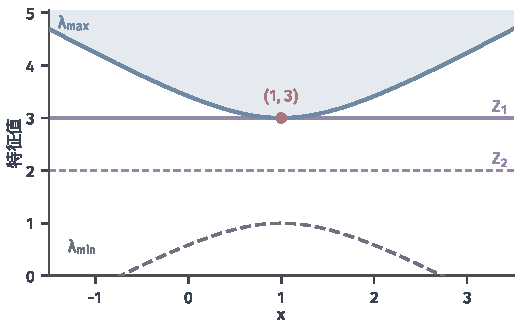
\includegraphics[width=88mm]{figures/05-optimization/06-constrained-optimization/matplotlib/cone-sdp-spectral/figure.pdf}
  \caption{$\bm{B}(x)$的两个特征值。浅蓝区域是$\lambda_{\max}(\bm{B}(x))\leq t$的$(x,t)$，红点是最优解。紫色实线$Z_1$是由$\bm{Z}_1=\frac12\begin{bmatrix}1&1\\1&1\end{bmatrix}$给出的下界$3$，紫色虚线$Z_2$是由$\bm{Z}_2=\frac12\bm{I}$给出的下界$2$。}
  \label{fig:cone-sdp-spectral}
\end{BookInlineFigure}

\subsection{锥对偶与证书}
\label{sec:cone-duality-certificates}

对偶问题~\eqref{eq:cone-conic-dual}要用到$\bm{K}^*$。这一小节算出三种常用锥的对偶锥，写出对应的对偶问题，再说明弱对偶可以放心使用，而强对偶需要额外的条件。

\paragraph{自对偶性}
下面的定理说，这三种锥的乘子就在原来的锥里取。

\begin{theorem}[三种常用锥的自对偶性]
\label{thm:cone-self-dual}
$\mathbb{R}^n_+$、$\bm{K}_{\mathrm{so}}^{k+1}$和$\mathcal{S}^n_+$的对偶锥都是它们自身。其中$\mathcal{S}^n_+$的内积取迹内积。
\end{theorem}

\begin{proof}
\emph{非负象限。}若$\bm{s}\geq\bm{0}$，对$\bm{x}\geq\bm{0}$有$\bm{s}^\top\bm{x}\geq0$。反过来，若$s_i<0$，取$\bm{x}=\bm{e}_i$得$\bm{s}^\top\bm{x}<0$。

\emph{二阶锥。}设$(\bm{v},w)$、$(\bm{u},t)$都在二阶锥中。由Cauchy--Schwarz不等式，
\[
 \bm{v}^\top\bm{u}+wt\geq-\lVert\bm{v}\rVert_2\lVert\bm{u}\rVert_2+wt\geq-wt+wt=0.
\]
所以二阶锥包含于它的对偶锥。

反过来，设$(\bm{v},w)$在对偶锥中。取$(\bm{u},t)=(\bm{0},1)$，得$w\geq0$。若$\bm{v}\neq\bm{0}$，取$\bm{u}=-\bm{v}/\lVert\bm{v}\rVert_2$、$t=1$，得到$-\lVert\bm{v}\rVert_2+w\geq0$。这两种情形都给出$\lVert\bm{v}\rVert_2\leq w$。

\emph{半正定锥。}设$\bm{X},\bm{S}\succeq\bm{0}$，由谱分解取半正定平方根，
\[
 \langle\bm{S},\bm{X}\rangle=\operatorname{tr}(\bm{S}^{1/2}\bm{X}\bm{S}^{1/2})\geq0,
\]
因为$\bm{S}^{1/2}\bm{X}\bm{S}^{1/2}$半正定，迹就是非负特征值之和。

反过来，设$\bm{S}$在对偶锥中。对任意$\bm{v}$，取$\bm{X}=\bm{v}\bm{v}^\top\succeq\bm{0}$，得到
\[
 \langle\bm{S},\bm{v}\bm{v}^\top\rangle=\bm{v}^\top\bm{S}\bm{v}\geq0,
\]
所以$\bm{S}\succeq\bm{0}$。
\end{proof}

半正定锥的乘子是半正定矩阵，不是元素非负的矩阵；二阶锥的乘子也有分量可以为负。线性规划里“乘子非负”这句话，推广之后是“乘子属于对偶锥”。

\paragraph{写出对偶问题}
把定理~\ref{thm:cone-self-dual}代入式~\eqref{eq:cone-conic-dual}。对二阶锥规划~\eqref{eq:cone-socp}，每条约束对应乘子$(\bm{u}_i,\tau_i)$，等式的乘子记作$\bm{y}$。按定义逐项写出，对偶问题是
\begin{equation}
 \begin{aligned}
 \max\quad&\bm{b}^\top\bm{y}-\sum_{i=1}^m(\bm{b}_i^\top\bm{u}_i+d_i\tau_i)\\
 \text{s.t.}\quad&\bm{A}^\top\bm{y}+\sum_{i=1}^m(\bm{A}_i^\top\bm{u}_i+\tau_i\bm{c}_i)=\bm{q},\\
 &\lVert\bm{u}_i\rVert_2\leq\tau_i,\quad i=1,\ldots,m.
 \end{aligned}
 \label{eq:cone-socp-dual}
\end{equation}

半正定规划~\eqref{eq:cone-sdp}中$\bm{X}$本身属于锥，相当于$\bm{E}$是恒等映射、$\bm{g}=\bm{0}$，对偶问题是
\begin{equation}
 \max_{\bm{y},\bm{S}}\ \bm{b}^\top\bm{y}\quad\text{s.t.}\quad\sum_{i=1}^my_i\bm{A}_i+\bm{S}=\bm{W},\quad\bm{S}\succeq\bm{0}.
 \label{eq:cone-sdp-dual}
\end{equation}
相应的间隙公式是
\begin{equation}
 \langle\bm{W},\bm{X}\rangle-\bm{b}^\top\bm{y}=\langle\bm{S},\bm{X}\rangle.
 \label{eq:cone-sdp-gap}
\end{equation}

\begin{example}[透镜问题的对偶证书]
\label{ex:cone-lens-dual}
对问题~\eqref{eq:cone-lens}，式~\eqref{eq:cone-socp-dual}成为：在$\bm{u}_1+\bm{u}_2=\bm{q}$、$\lVert\bm{u}_i\rVert_2\leq\tau_i$下最大化
\[
 \bm{a}_1^\top\bm{u}_1+\bm{a}_2^\top\bm{u}_2-5\tau_1-5\tau_2.
\]
先任取一个可行的乘子，看它给出什么下界。取$\bm{u}_1=\bm{u}_2=(0,1/2)$，$\tau_1=\tau_2=1/2$，对偶目标是$-5$。所以无论可行点是什么，$x_2\geq-5$，这个下界对，但不紧。

要使间隙为零，由式~\eqref{eq:cone-conic-gap}，每条约束的$(\bm{u}_i,\tau_i)$必须与$(\bm{x}^\star-\bm{a}_i,5)$内积为零。两个向量都在二阶锥的边界上时，这要求$\bm{u}_i$与$\bm{x}^\star-\bm{a}_i$反向，且$\lVert\bm{u}_i\rVert_2=\tau_i$。

在$\bm{x}^\star=(3,-4)$处，这给出
\[
 \bm{u}_1=\tau_1\begin{bmatrix}-3/5\\4/5\end{bmatrix},\qquad
 \bm{u}_2=\tau_2\begin{bmatrix}3/5\\4/5\end{bmatrix}.
\]
再由$\bm{u}_1+\bm{u}_2=(0,1)$，解得
\[
 \tau_1=\tau_2=\frac58,\qquad
 \bm{u}_1=\begin{bmatrix}-3/8\\1/2\end{bmatrix},\qquad
 \bm{u}_2=\begin{bmatrix}3/8\\1/2\end{bmatrix}.
\]
对偶目标是
\[
 0+\frac{18}{8}-\frac{25}{8}-\frac{25}{8}=-4.
\]
它等于原始目标值，所以$(3,-4)$最优，这对乘子也最优。图~\ref{fig:cone-soc-lens}中的紫色箭头画的就是$\bm{u}_1,\bm{u}_2$，二者之和是目标的梯度。
\end{example}

\begin{example}[谱上界的对偶证书]
\label{ex:cone-spectral-dual}
对$\min t$、$t\bm{I}-\bm{B}(x)\succeq\bm{0}$，取乘子$\bm{Z}\succeq\bm{0}$。不必套公式，直接从谱上界出发：任何$\operatorname{tr}\bm{Z}=1$的$\bm{Z}\succeq\bm{0}$都满足
\[
 \lambda_{\max}(\bm{B}(x))\geq\langle\bm{Z},\bm{B}(x)\rangle,
\]
因为$\lambda_{\max}\bm{I}-\bm{B}(x)\succeq\bm{0}$与$\bm{Z}$的迹内积非负。

若再选$\bm{Z}$使右端不含$x$，就得到一个对所有$x$成立的常数下界。$\bm{B}(x)$中$x$的系数是$\operatorname{diag}(1,-1)$，所以要求$Z_{1,1}=Z_{2,2}$，再由迹为$1$得$Z_{1,1}=Z_{2,2}=1/2$。取$Z_{1,2}=1/2$，得到
\[
 \bm{Z}_1=\frac12\begin{bmatrix}1&1\\1&1\end{bmatrix},\qquad
 \langle\bm{Z}_1,\bm{B}(x)\rangle=\frac12(1+x+2+3-x)=3.
\]
变量$x$消掉了，于是$\lambda_{\max}(\bm{B}(x))\geq3$对所有$x$成立。$x=1$时取等，这就是最优性的证明，即图~\ref{fig:cone-sdp-spectral}的紫色实线。

取$Z_{1,2}=0$，同样的计算给出常数$2$，下界正确但不紧，是图中的紫色虚线。
\end{example}

\paragraph{矩阵互补}
式~\eqref{eq:cone-conic-gap}说明，零间隙等价于$\bm{s}^\top(\bm{E}\bm{x}+\bm{g})=0$，这是互补松弛的锥形式。半正定时，这个条件比一个数等于零更强。

设$\bm{X},\bm{S}\succeq\bm{0}$且$\langle\bm{S},\bm{X}\rangle=0$，则
\[
 \operatorname{tr}(\bm{S}^{1/2}\bm{X}\bm{S}^{1/2})=\lVert\bm{X}^{1/2}\bm{S}^{1/2}\rVert_{\mathrm{F}}^2=0.
\]
所以$\bm{X}^{1/2}\bm{S}^{1/2}=\bm{0}$，再两边分别乘$\bm{X}^{1/2}$和$\bm{S}^{1/2}$，得到
\begin{equation}
 \bm{X}\bm{S}=\bm{0}.
 \label{eq:cone-matrix-complementarity}
\end{equation}
二者的列空间互相正交，秩之和不超过$n$。

以迹为$1$的例子验证。对偶问题是$\max y$、$\bm{S}=\bm{W}-y\bm{I}\succeq\bm{0}$，最优值在$y=\lambda_{\min}(\bm{W})=1$取得。这时
\[
 \bm{S}=\begin{bmatrix}1&1\\1&1\end{bmatrix},\qquad
 \bm{X}^\star\bm{S}=\frac12\begin{bmatrix}1&-1\\-1&1\end{bmatrix}\begin{bmatrix}1&1\\1&1\end{bmatrix}=\bm{0}.
\]

\paragraph{强对偶需要条件}
弱对偶无条件成立，证书就是这么来的。但两个目标值是否一定能碰到一起？线性规划中，只要原始和对偶都可行，最优值就相等且都能取到。这一结论不能原样推广。

类似第~\ref{chap:duality}章的Slater条件，锥规划也有严格可行性的条件。若存在满足$\bm{A}\bm{x}=\bm{b}$且$\bm{E}\bm{x}+\bm{g}\in\operatorname{int}\bm{K}$的点，并且原始最优值有限，则对偶问题取得最优解，且间隙为零。把原始和对偶的角色对调，结论同样成立。证明用凸集分离定理，与Slater条件的论证相同，只是把标量不等式换成锥成员条件，读者可查阅凸优化教材\scite{math-boyd2004convex}。

下面两个例子说明缺少这一条件时会出什么问题。

\begin{example}[最优值取不到]
\label{ex:cone-non-attain}
考虑
\[
 \min_{\bm{x}}\ x_1\quad\text{s.t.}\quad\begin{bmatrix}x_1&1\\1&x_2\end{bmatrix}\succeq\bm{0}.
\]
约束等价于$x_1,x_2>0$且$x_1x_2\geq1$，可行集是双曲线上方的区域，如图~\ref{fig:cone-sdp-gaps}(a)所示。取$x_1=1/k$、$x_2=k$，目标趋于$0$，但$x_1=0$不可行，最优值$0$取不到。

把式~\eqref{eq:cone-conic-dual}写出来：$\bm{Z}\succeq\bm{0}$，$Z_{1,1}=1$，$Z_{2,2}=0$，目标是$-2Z_{1,2}$。半正定和$Z_{2,2}=0$迫使$Z_{1,2}=0$，对偶唯一的可行值是$0$，它取到了。

这里原始严格可行（取$x_1=x_2=2$），所以对偶取得最优且间隙为零，符合上面的结论。对偶没有严格可行点，所以原始不保证取得最优解。
\end{example}

\begin{example}[正的对偶间隙]
\label{ex:cone-positive-gap}
考虑
\[
 \min_{\bm{x}}\ x_1\quad\text{s.t.}\quad\begin{bmatrix}0&x_1&0\\x_1&x_2&0\\0&0&x_1+1\end{bmatrix}\succeq\bm{0}.
\]
半正定矩阵的对角元为零时，同行同列都为零，所以$x_1=0$，$p^\star=0$。

对偶问题的乘子$\bm{Z}\succeq\bm{0}$要满足两个条件。$x_2$的系数给出$Z_{2,2}=0$，从而$Z_{1,2}=0$。$x_1$的系数给出$2Z_{1,2}+Z_{3,3}=1$，从而$Z_{3,3}=1$。

对偶目标是$-Z_{3,3}=-1$，所以$d^\star=-1$。原始和对偶都可行，也都取到最优值，二者却相差$1$，见图~\ref{fig:cone-sdp-gaps}(b)。原始可行集的矩阵全部奇异，严格可行性不成立。
\end{example}

\begin{BookInlineFigure}
  \centering
  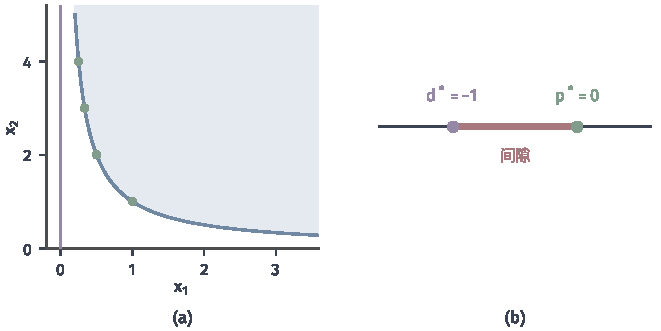
\includegraphics[width=112mm]{figures/05-optimization/06-constrained-optimization/matplotlib/cone-sdp-gaps/figure.pdf}
  \caption{半正定规划强对偶失效的两种方式。(a)浅蓝区域是可行集$x_1x_2\geq1$，绿点$(1/k,k)$的目标趋于紫线$x_1=0$，但永远到不了。(b)原始最优值$0$（绿）与对偶最优值$-1$（紫）之间有正间隙（红）。}
  \label{fig:cone-sdp-gaps}
\end{BookInlineFigure}

这些现象的根源在于，闭凸锥在线性映射下的像不一定闭。非负象限是多面体，多面体的线性像仍是闭集，二阶锥和半正定锥则没有这个保证。表~\ref{tab:cone-duality-compare}归纳了差别。

\begin{BookInlineTable}
  \centering
  \begin{tabular}{lll}
    \toprule
    性质 & 线性规划 & 一般锥规划\\
    \midrule
    弱对偶 & 成立 & 成立\\
    两边可行时间隙为零 & 成立 & 不一定\\
    最优值能取到 & 有限时取到 & 不一定\\
    零间隙的依据 & 无需额外条件 & 严格可行性等条件\\
    \bottomrule
  \end{tabular}
  \caption{线性规划与一般锥规划的对偶性质对比。}
  \label{tab:cone-duality-compare}
\end{BookInlineTable}

所以报告半正定规划的结果时，弱对偶给出的界永远可靠；“间隙为零”这句话则要么由算出的两个可行解直接验证，要么先核对严格可行性。
